\documentclass[conference]{IEEEtran}
\usepackage{graphicx}
\usepackage{booktabs}
\usepackage{amsmath}
\usepackage{hyperref}
\usepackage{subcaption}
\usepackage{caption}

\captionsetup{font=footnotesize}
\setlength{\textfloatsep}{6pt plus 2pt minus 2pt}
\setlength{\floatsep}{4pt plus 2pt minus 2pt}
\setlength{\intextsep}{6pt plus 2pt minus 2pt}

% Urdu script for qualitative translation examples. fontspec is used only
% to declare one extra family; the document body font is untouched.
\usepackage{fontspec}
\newfontfamily\urdufont{Noto Nastaliq Urdu}[Script=Arabic]

\begin{document}

\title{Two Studies in Data-Constrained Deep Learning: Chest X-ray Classification and English--Urdu Neural Translation}

\author{
\IEEEauthorblockN{Soban Ahmad}
\IEEEauthorblockA{FAST National University of Computer and Emerging Sciences\\
sobanahmad2003@gmail.com}
}

\maketitle

\begin{abstract}
We report two independent studies. In Q1, a custom 1.24M-parameter CNN
(PneumoNet) is trained from scratch to classify chest radiographs into
COVID-19, Normal, and Pneumonia, and compared against frozen and
fine-tuned VGG16 and ResNet50 baselines under identical conditions.
PneumoNet outperforms all four pre-trained baselines on every test metric
(accuracy 0.9797, macro-F1 0.9794, macro-AUC 0.9982), including
fine-tuned VGG16 at 108$\times$ the parameter count. In Q2, a vanilla
RNN encoder--decoder (no attention, no gating) is trained on an
English--Urdu sentence-pair corpus for neural machine translation; the
originally reported result was diagnosed as under-trained rather than
constraint-limited, and correcting the teacher-forcing schedule
together with reversing the source sequence raises test BLEU from 2.45
to 4.64, though the corrected model remains fluent but largely
unfaithful to its source. Both studies surface measurement-driven
findings that contradict default assumptions in the respective
pipelines: a duplicate-detection threshold imported from natural-image
practice fails on chest radiographs, horizontal flipping corrupts a
laterality marker, frozen backbones silently adapt through BatchNorm
statistics, an L2 regularization sweep is numerically inert at float32
precision, a Q2 quality ceiling initially attributed to the
no-attention architecture was actually an under-trained
teacher-forcing configuration, and the Q2 corpus is a ninth of the
assignment's stated size and overwhelmingly Biblical in register.
\end{abstract}

\section{Introduction}

\subsection{Q1: Chest X-ray Classification}
Automated triage of chest radiographs into COVID-19, Normal, and
Pneumonia classes is a natural fit for CNNs, but production pipelines
default to large ImageNet-pretrained backbones without asking whether a
small, task-specific network trained from scratch might do as well with
far fewer parameters and no transfer-learning risk. This study builds
PneumoNet, a 1,239,779-parameter CNN, and benchmarks it against frozen
and fine-tuned VGG16 (134.3M params) and ResNet50 (23.5M params) under
identical data, splits, and training budget. Contributions: a
calibrated near-duplicate detection procedure for radiographs (Section
II), a measured augmentation policy rather than an assumed one (Section
IV), a BatchNorm-freezing correction that changes what "frozen baseline"
actually means (Section III), and a full grid-search-tuned comparison
showing the small model wins (Section V).

\subsection{Q2: English--Urdu Neural Machine Translation}
A vanilla RNN encoder--decoder is the base case against which attention
and gating are usually justified, but that justification is rarely
measured directly, and rarely disentangled from ordinary training
bugs. This study trains an \texttt{nn.RNN}-only encoder--decoder (no
LSTM, GRU, attention, or Transformer component) on an English--Urdu
parallel corpus and evaluates it with BLEU, length-bucketed BLEU, and
an error taxonomy. Contributions: an audit of the actual corpus against
the assignment's description (Section II); a three-configuration sweep
that diagnoses the originally reported quality ceiling as
under-training (a static 0.5 teacher-forcing rate and forward-order
source) rather than architecture, and corrects it, nearly doubling test
BLEU (Section IV); and evidence that, even after correction,
translation quality remains bounded not by sentence length but by the
single fixed-size hidden vector's ability to condition generation
faithfully on the source (Section VI).

\section{Dataset and Preprocessing}

\subsection{Q1}
The source is the Kaggle \texttt{prashant268/chest-xray-covid19-pneu\-monia}
dataset: 6,432 images across three classes, all decodable (0 corrupt).
Near-duplicate detection was recalibrated during development. An
initial dHash-8/Hamming-distance-$\leq 3$ rule flagged 1,570 of 6,432
images (25\%) as near-duplicates; a 40-pair audit of the flagged set
found zero genuinely near-identical pairs, a mean flagged-pair
correlation of 0.842 against a random-pair baseline of 0.605, and 10 of
40 flagged pairs spanning two different diagnostic classes. The root
cause: chest radiographs share gross anatomy and framing, so the
dataset-wide median nearest-neighbour thumbnail correlation is already
0.926 (p99 0.970, p99.5 0.987) --- a perceptual-hash threshold
calibrated on natural images does not transfer to this domain. The rule
was replaced with contrast-normalized $32\times32$-thumbnail
correlation $\geq 0.99$, which sits in the genuine-duplicate tail and
removes 34 exact plus 15 near duplicates, 49 of 6,432 images (0.76\%).
One of the removed near-duplicate pairs crosses diagnostic classes:
\texttt{PNEUMONIA(7).jpg} (dropped) and \texttt{COVID19(277).jpg}
(kept) correlate at 0.9913 --- the same radiograph filed under two
different diagnoses in the raw data, measured label noise that
deduplication can silence but not resolve, since which of the two
original labels was correct is unknowable from the image alone. The
kept manifest (6,383 images: COVID19
560, Normal 1{,}579, Pneumonia 4{,}244) is split 80/10/10, stratified by
class, giving train/val/test = 5{,}106/638/639 images, a 7.6:1
Pneumonia-to-COVID19 imbalance carried into a weighted loss (Section
III). Augmentation policy was measured, not assumed: Fig.~\ref{fig:aug}
shows that horizontal flipping mirrors the radiopaque \texttt{R}
laterality marker into a mirrored, Cyrillic-``ya''-shaped artifact --- not
just anatomically questionable for a chest film, but a visible,
class-irrelevant shortcut cue an augmented model could exploit.

\begin{figure}[t]
\centering
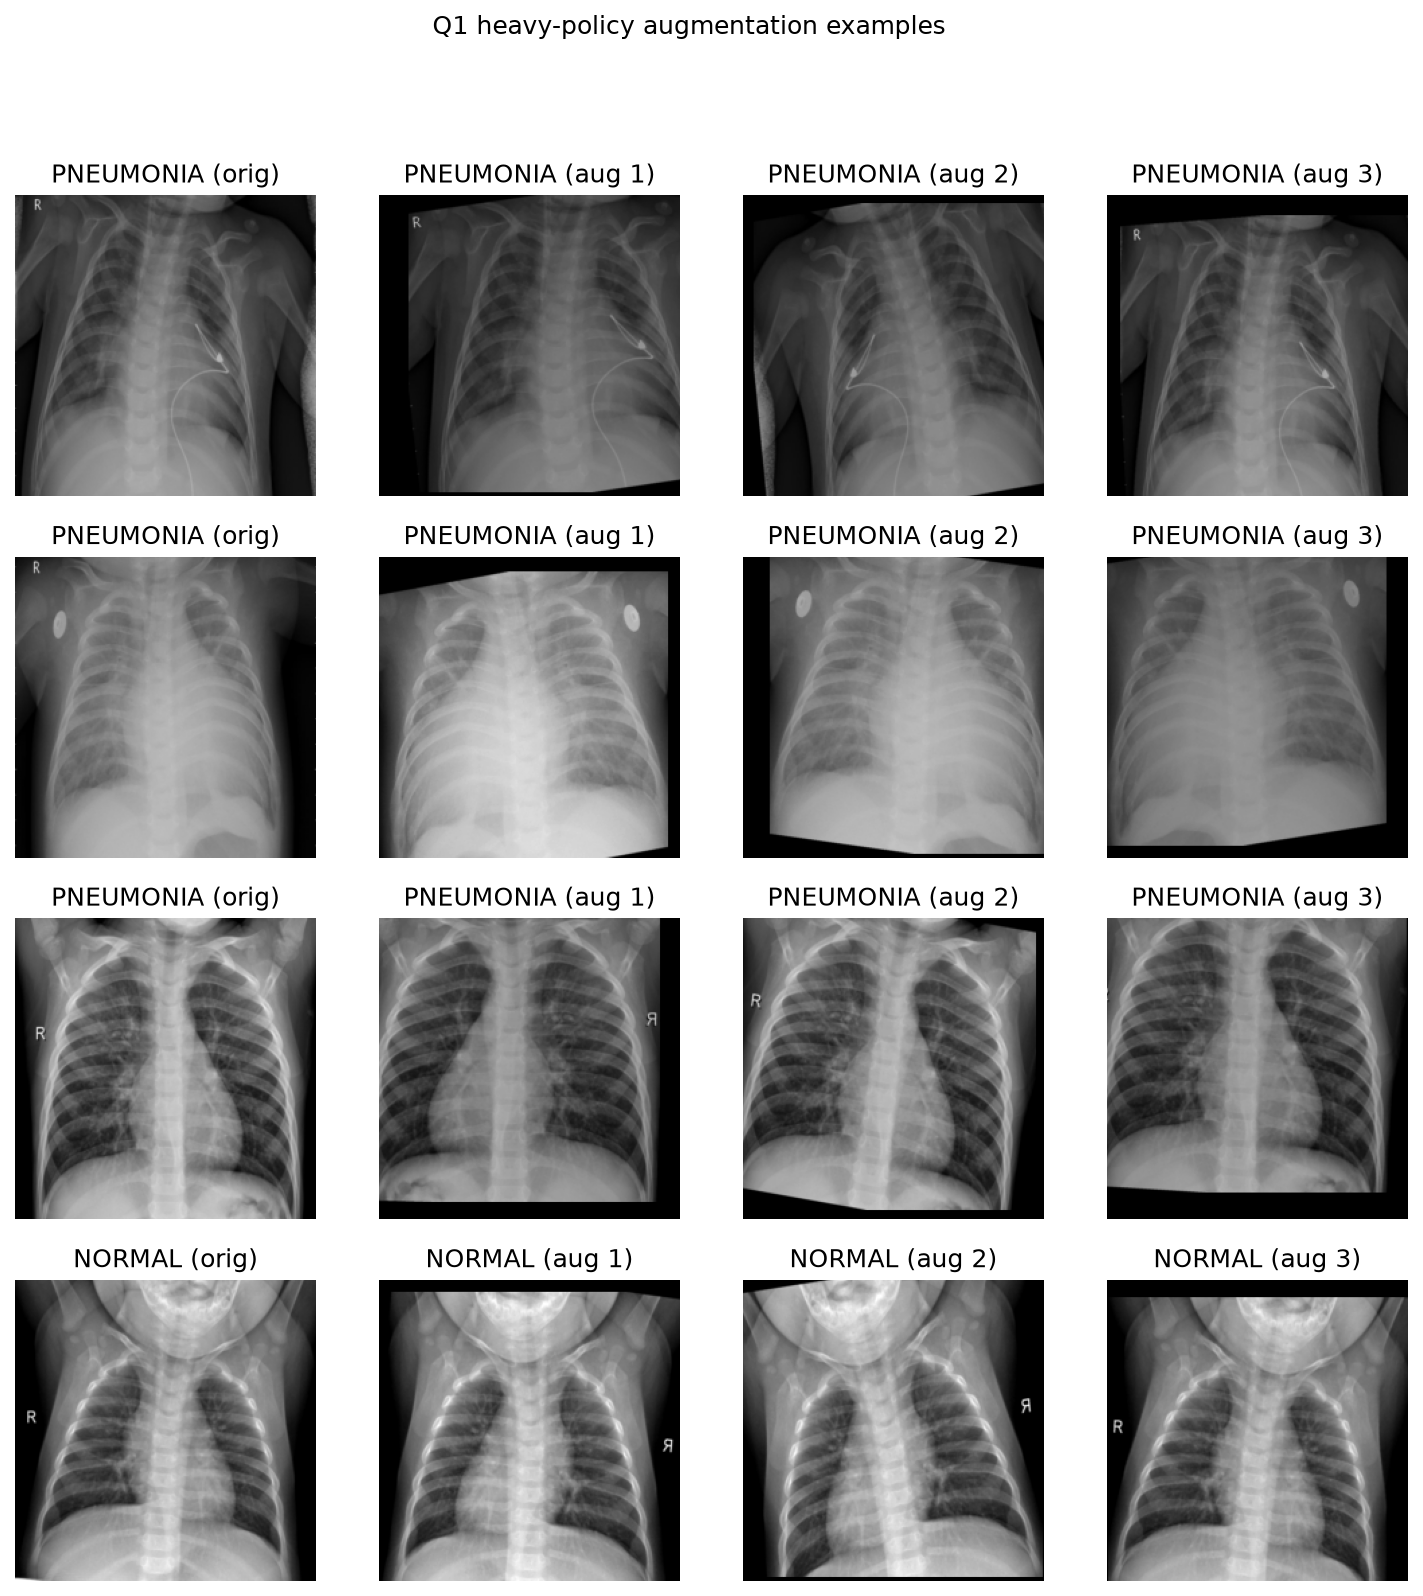
\includegraphics[width=\linewidth]{../results/figs/q1_augmentation.png}
\caption{Heavy-policy augmentation examples. Rows 3--4 show the R laterality marker mirrored into a Cyrillic-``ya''-shaped artifact under horizontal flip.}
\label{fig:aug}
\end{figure}

\subsection{Q2}
The source is the Kaggle \texttt{muhammadnoman76/translation-dataset}
English--Urdu spreadsheet. The assignment describes a corpus of
approximately 24,000 general parallel sentence pairs; the file actually
delivered contains \textbf{9,103} pairs in a single sheet. Word-level
auditing of the raw English side shows the corpus is overwhelmingly
Biblical text in King James register: ``unto'' appears in 22.7\% of
sentences, ``god'' 13.1\%, ``shall'' 11.0\%, ``jesus'' 10.4\%,
``thou''/``thee''/``thy'' in 6.8\%/4.3\%/3.4\%, over 6,561 unique
English word types across 187,640 tokens --- extremely repetitive, with
a small modern-conversational tail late in the file. Preprocessing
NFC-normalizes and lowercases English, folds Arabic-form Urdu
characters to Urdu forms (deliberately excluding alef-with-madda, a
distinct Urdu letter, from that folding), strips diacritics, and
separates punctuation into its own tokens. Cleaning drops 1 empty and 10 exact-duplicate
pairs (9,092 kept), and a length filter (95th-percentile per-side token
cap, max length ratio 2.5) removes a further 627 long and 25
skewed-ratio pairs, leaving 8,440 pairs split 80/10/10
(6,752/844/844, unstratified --- no labels to stratify on).
Word-level vocabularies (min. frequency 2) give 3,656 source and 3,961
target types, with validation OOV rates of 3.18\% (English) and 3.50\%
(Urdu).

\section{Methodology}

\subsection{Q1}
PneumoNet (Table~\ref{tab:pneumonet}, 1,239,779 params) is four
convolutional blocks doubling channels $32\to64\to128\to256$, each
block two Conv-BatchNorm-ReLU \cite{ioffe2015batchnorm} pairs followed
by max-pooling, then global average pooling and a dropout-regularized
two-layer classifier head.

\begin{table}[htbp]
\centering
\caption{PneumoNet architecture: layer types, output shapes and parameter counts.}
\label{tab:pneumonet}
\begin{tabular}{llr}
\hline
Layer & Output Shape & Parameters \\
\hline
PneumoNet & [1, 3] & 1,239,779 \\
Sequential: 1-1 & [1, 256, 14, 14] & 1,173,216 \\
Sequential: 2-1 & [1, 32, 112, 112] & 10,208 \\
Conv2d: 3-1 & [1, 32, 224, 224] & 864 \\
BatchNorm2d: 3-2 & [1, 32, 224, 224] & 64 \\
ReLU: 3-3 & [1, 32, 224, 224] & -- \\
Conv2d: 3-4 & [1, 32, 224, 224] & 9,216 \\
BatchNorm2d: 3-5 & [1, 32, 224, 224] & 64 \\
ReLU: 3-6 & [1, 32, 224, 224] & -- \\
MaxPool2d: 3-7 & [1, 32, 112, 112] & -- \\
Sequential: 2-2 & [1, 64, 56, 56] & 55,552 \\
Conv2d: 3-8 & [1, 64, 112, 112] & 18,432 \\
BatchNorm2d: 3-9 & [1, 64, 112, 112] & 128 \\
ReLU: 3-10 & [1, 64, 112, 112] & -- \\
Conv2d: 3-11 & [1, 64, 112, 112] & 36,864 \\
BatchNorm2d: 3-12 & [1, 64, 112, 112] & 128 \\
ReLU: 3-13 & [1, 64, 112, 112] & -- \\
MaxPool2d: 3-14 & [1, 64, 56, 56] & -- \\
Sequential: 2-3 & [1, 128, 28, 28] & 221,696 \\
Conv2d: 3-15 & [1, 128, 56, 56] & 73,728 \\
BatchNorm2d: 3-16 & [1, 128, 56, 56] & 256 \\
ReLU: 3-17 & [1, 128, 56, 56] & -- \\
Conv2d: 3-18 & [1, 128, 56, 56] & 147,456 \\
BatchNorm2d: 3-19 & [1, 128, 56, 56] & 256 \\
ReLU: 3-20 & [1, 128, 56, 56] & -- \\
MaxPool2d: 3-21 & [1, 128, 28, 28] & -- \\
Sequential: 2-4 & [1, 256, 14, 14] & 885,760 \\
Conv2d: 3-22 & [1, 256, 28, 28] & 294,912 \\
BatchNorm2d: 3-23 & [1, 256, 28, 28] & 512 \\
ReLU: 3-24 & [1, 256, 28, 28] & -- \\
Conv2d: 3-25 & [1, 256, 28, 28] & 589,824 \\
BatchNorm2d: 3-26 & [1, 256, 28, 28] & 512 \\
ReLU: 3-27 & [1, 256, 28, 28] & -- \\
MaxPool2d: 3-28 & [1, 256, 14, 14] & -- \\
AdaptiveAvgPool2d: 1-2 & [1, 256, 1, 1] & -- \\
Sequential: 1-3 & [1, 3] & 66,563 \\
Flatten: 2-5 & [1, 256] & -- \\
Dropout: 2-6 & [1, 256] & -- \\
Linear: 2-7 & [1, 256] & 65,792 \\
ReLU: 2-8 & [1, 256] & -- \\
Dropout: 2-9 & [1, 256] & -- \\
Linear: 2-10 & [1, 3] & 771 \\
\hline
Total & & 1,239,779 \\
\hline
\end{tabular}
\end{table}


The four baselines are ImageNet-pretrained VGG16 \cite{simonyan2015vgg}
and ResNet50 \cite{he2016resnet}, each run frozen (only a new head
trained) and fine-tuned (VGG16: last convolutional block unfrozen;
ResNet50: \texttt{layer4} unfrozen), so ten total configurations
reduce to the five reported after selecting one setting per
architecture pairing shown in Table~\ref{tab:q1comparison}. A
correction was required for the frozen baselines:
\texttt{requires\_grad=False} blocks gradient updates to BatchNorm
affine parameters but does not stop BatchNorm from updating its
\texttt{running\_mean}/\texttt{running\_var} buffers in \texttt{train()}
mode, since that update is unconditional on \texttt{requires\_grad}. On
\texttt{resnet50\_frozen}, one measured forward/backward/optimizer step
moved \texttt{bn1.running\_mean} by 0.1565 before the fix and exactly
0.0 after forcing frozen BatchNorm modules to stay in \texttt{eval()}
mode across every \texttt{train()} call. Without this fix, "frozen"
baselines would have silently adapted their BatchNorm statistics to the
chest X-ray domain every epoch, inflating their scores and
understating the frozen-vs-fine-tuned gap Section V reports.

\subsection{Q2}
The encoder--decoder \cite{sutskever2014seq2seq}
(Table~\ref{tab:q2seq2seqlayers}, 4,770,425 params) uses
\texttt{nn.RNN} with tanh nonlinearity exclusively --- no LSTM, GRU,
attention module, or Transformer component anywhere in the model, a
hard constraint of the study rather than a design preference, so that
Section VI can characterize what a single fixed-size hidden vector can
and cannot carry.

\begin{table}[htbp]
\centering
\scriptsize
\caption{Q2 vanilla RNN encoder--decoder: layer parameter shapes (src\_vocab=3656, tgt\_vocab=3961).}
\label{tab:q2seq2seqlayers}
\begin{tabular}{lp{3.4cm}r}
\hline
Layer & Parameter Shapes & Parameters \\
\hline
encoder.embedding & (3656, 256) & 935,936 \\
encoder.rnn & (512, 256), (512, 512), (512,), (512,) & 394,240 \\
decoder.embedding & (3961, 256) & 1,014,016 \\
decoder.rnn & (512, 256), (512, 512), (512,), (512,) & 394,240 \\
decoder.fc\_out & (3961, 512), (3961,) & 2,031,993 \\
\hline
Total & & 4,770,425 \\
\hline
\end{tabular}
\end{table}


The encoder packs its embedded input with
\texttt{pack\_padded\_sequence} (\texttt{enforce\_sorted=False}) before
the recurrence so PAD steps never contaminate the final hidden state
handed to the decoder. Decoder inputs and targets are built under an
explicit shifting contract: for target tokens $[w_1, w_2]$,
$\texttt{dec\_in} = [\texttt{SOS}, w_1, w_2, \texttt{PAD}\ldots]$ and
$\texttt{dec\_target} = [w_1, w_2, \texttt{EOS}, \texttt{PAD}\ldots]$,
with a masked cross-entropy loss (Section IV) ignoring PAD positions on
the target side.

\section{Experimental Setup}

\subsection{Q1}
All models train with AdamW \cite{loshchilov2019adamw}, a
class-weighted loss (inverse label frequency) for the 7.6:1 imbalance,
and early stopping on validation macro-F1. Hyperparameters were
selected by staged coordinate descent over 30 proxy configurations at
$128\times128$ resolution (stages A: augmentation$\times$normalization,
B: batch size$\times$lr, C1--C3: dropout, L2, L1, D:
epochs$\times$patience), not an exhaustive Cartesian product --- a full
grid over these axes would run into days of MPS wall time, which the
project's compute budget did not allow. Table~\ref{tab:q1hyper} reports
the searched range and selected value for every axis.

\begin{table}[htbp]
\centering
\small
\caption{Grid search: hyperparameter, range searched, and optimal value.}
\label{tab:q1hyper}
\begin{tabular}{lll}
\hline
hyperparameter & range & optimal \\
\hline
augmentation & heavy, light, none & none \\
normalization & dataset, imagenet, zero\_one & imagenet \\
batch\_size & 16, 32, 64 & 16 \\
lr & 0.0001, 0.0003, 0.001 & 0.0001 \\
dropout & 0.2, 0.3, 0.5 & 0.3 \\
l2\_lambda & 0, 1e-05, 0.0001 & 0 \\
l1\_lambda & 0, 1e-05 & 0 \\
epochs & 30, 60 & 60 \\
patience & 5, 10 & 10 \\
\hline
\end{tabular}
\end{table}


Two results are reported honestly rather than smoothed over. First, augmentation: stage A shows augmentation monotonically
\emph{hurting} validation macro-F1 across all three normalization
schemes without exception (none $>$ light $>$ heavy; best
none+imagenet 0.9745, worst heavy+dataset 0.9508), consistent with
Section II's finding that this dataset is clean, consistently framed,
and harmed rather than helped by geometric invariance training.
Second, L2 weight decay: the searched range
$\{0, 10^{-5}, 10^{-4}\}$ returned bit-identical validation macro-F1
(0.9756799123668505) for all three values in stage C2. This is not a
discreteness artifact of the metric; an isolated 200-step AdamW
experiment at the same learning rate reproduces it directly ---
$\lambda\in\{0, 10^{-5}, 10^{-4}\}$ give identical loss and weights,
while $\lambda=10^{-2}$ differs. AdamW's decoupled update
$p \leftarrow p - \eta\lambda p$ at $\eta=10^{-4}$, $\lambda=10^{-4}$
is a relative per-step change of $10^{-8}$, below float32 epsilon
($\approx 1.19\times10^{-7}$), so it rounds to exactly no change: the
searched range was below representable precision, a trap for any
small-weight-decay/small-learning-rate float32 experiment. The searched
range and optimal value ($\lambda=0$) are reported as-is in
Table~\ref{tab:q1hyper}. The search's own top selection for
epochs/patience was 60/10 (validation macro-F1 0.9761, 49 epochs run),
narrowly ahead of 30/5 (0.9757, 17 epochs) --- a gain of 0.0004 for
roughly 3$\times$ the compute. Under a stated compute budget, the five
full-size runs reported in Section V used 30/5, not the search's
60/10 selection; both numbers are reported here so the near-tie between
configurations 3$\times$ apart in cost stands as a tuning observation
in its own right, not a discrepancy to hide. All five full runs,
including VGG16 fine-tuning, completed at the winning batch size of 16
with no MPS out-of-memory event, so the pre-registered batch-size
fallback was not needed. Because Metal (MPS) kernels are not
bitwise-deterministic, splits, vocabularies, and every selected
hyperparameter reproduce exactly across runs, while metric values
reproduce to roughly $\pm0.3\%$; the seed is 42 throughout, set once in
a shared \texttt{set\_seed} utility.

\subsection{Q2}
Training minimizes masked cross-entropy (PAD positions excluded) with
Adam and gradient-norm clipping at 1.0. Clipping is genuinely active
early in training: 16\% of batches were clipped in epoch 1 (mean
pre-clip norm 0.815, max 1.702), falling below 1\% of batches by epoch
2 (mean pre-clip norm 0.693, max 1.068) --- evidence the vanilla RNN
has a real, if modest, gradient-explosion tendency that clipping is
actively controlling, not a ceremonial safeguard.

The originally reported model (test BLEU 2.45) was diagnosed as
\emph{under-trained}, not constraint-limited: it could not reproduce
training pairs it had already seen 32 times, and \texttt{train\_loss}
(4.297) exceeded \texttt{val\_loss} (4.244) --- a positive gap
characteristic of underfitting, not the capacity ceiling a hidden-vector
bottleneck would produce. Two configuration causes, not architectural
ones, were identified and fixed. First, \texttt{teacher\_forcing} was
fixed at 0.5 from epoch 1, so the decoder consumed its own untrained
predictions half the time and never received a clean training signal.
Second, the source sequence was fed in forward order; reversing it
\cite{sutskever2014seq2seq} shortens the dependency between the first
source and first target words, the standard remedy for an
attention-free RNN encoder--decoder. Table~\ref{tab:q2tuning} reports
all three measured configurations. Correcting teacher forcing alone
\emph{lowered} test BLEU (2.45$\to$1.56) even though it improved
validation perplexity (68.08$\to$57.76); only combined with source
reversal did BLEU nearly double, to 4.64, with perplexity falling
further to 53.37 --- perplexity and BLEU did not move together across
this sweep, worth noting honestly rather than smoothing into a single
trend line. \texttt{reverse\_source} changes token order only: it adds
no LSTM, GRU, attention, or Transformer component, so the vanilla-RNN
constraint stated in Section III still holds for the reported (final)
configuration. Under that corrected configuration, training ran 18
epochs to an early-stopping halt (configured budget 80/patience 8),
4,770,425 parameters, 210.3s total.

\begin{table}[htbp]
\centering
\scriptsize
\caption{Q2 tuning sweep: teacher forcing and source order (val. perplexity, test BLEU).}
\label{tab:q2tuning}
\begin{tabular}{lrr}
\hline
Configuration & Val. Perplexity & Test BLEU \\
\hline
TF=0.5, forward source (orig.) & 68.08 & 2.45 \\
TF=1.0, forward source & 57.76 & 1.56 \\
\textbf{TF=1.0, reversed source (final)} & \textbf{53.37} & \textbf{4.64} \\
\hline
\end{tabular}
\end{table}


\section{Results}

\subsection{Q1}
Table~\ref{tab:q1comparison} is the full cross-model test-set
comparison. PneumoNet leads on every metric: accuracy 0.9797, macro-F1
0.9794, macro-AUC 0.9982, against fine-tuned VGG16 (0.9765/0.9759/0.9980,
134.3M params) and fine-tuned ResNet50 (0.9734/0.9753/0.9949, 23.5M
params). Frozen baselines trail badly --- VGG16-frozen macro-F1
0.9160, ResNet50-frozen 0.9407 --- confirming ImageNet features
transfer weakly onto grayscale radiographs without adaptation.

\begin{table*}[t]
\centering
\small
\caption{Cross-model comparison on the held-out Q1 test split.}
\label{tab:q1comparison}
\begin{tabular}{lrrrrrr}
\hline
model & params (total) & params (trainable) & epoch time (s) & test acc. & test macro-F1 & test macro-AUC \\
\hline
pneumonet & 1239779 & 1239779 & 50.1662 & 0.9797 & 0.9794 & 0.9982 \\
vgg16\_frozen & 134272835 & 12291 & 61.4905 & 0.9249 & 0.9160 & 0.9836 \\
vgg16\_finetune & 134272835 & 7091715 & 72.3212 & 0.9765 & 0.9759 & 0.9980 \\
resnet50\_frozen & 23514179 & 6147 & 34.6194 & 0.9405 & 0.9407 & 0.9925 \\
resnet50\_finetune & 23514179 & 14970883 & 48.4463 & 0.9734 & 0.9753 & 0.9949 \\
\hline
\end{tabular}
\end{table*}


Fig.~\ref{fig:q1results} shows the normalized confusion matrix, ROC
curves, and training curves for PneumoNet. The data-volume study
(Fig.~\ref{fig:datavol}) trains PneumoNet on 25/50/75/100\% of the
training data: test macro-F1 is 0.9517 (25\%, $n=1{,}277$), 0.9670
(50\%, $n=2{,}554$), 0.9794 (75\%, $n=3{,}829$), and 0.9776 (100\%,
$n=5{,}106$) --- performance saturates at 75\%; the final quarter of
training data adds nothing, and the 100\% result is marginally lower,
within run-to-run noise, not a monotonic climb.

\begin{figure}[t]
\centering
\begin{subfigure}[b]{0.48\linewidth}
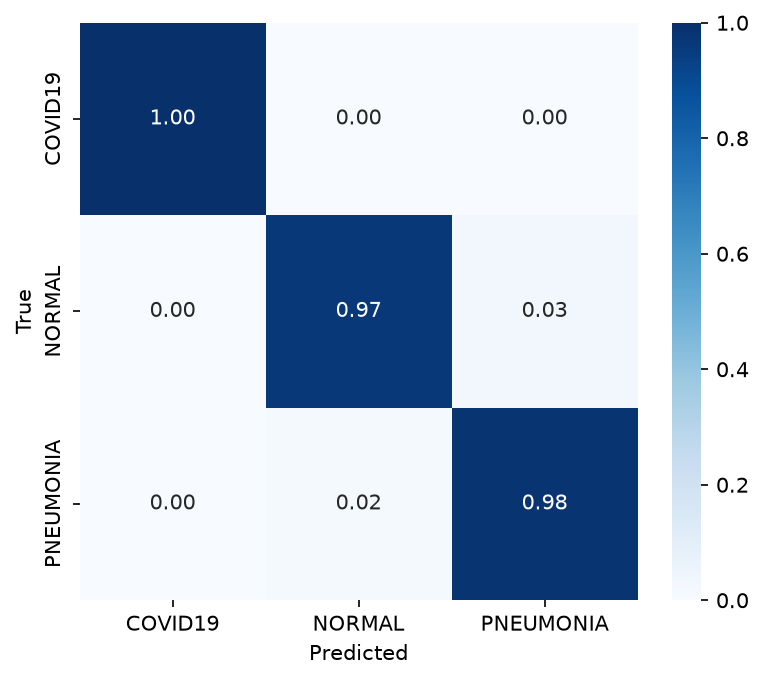
\includegraphics[width=\linewidth]{../results/figs/q1_confusion_matrix_norm.png}
\caption{Normalized confusion matrix}
\end{subfigure}
\hfill
\begin{subfigure}[b]{0.48\linewidth}
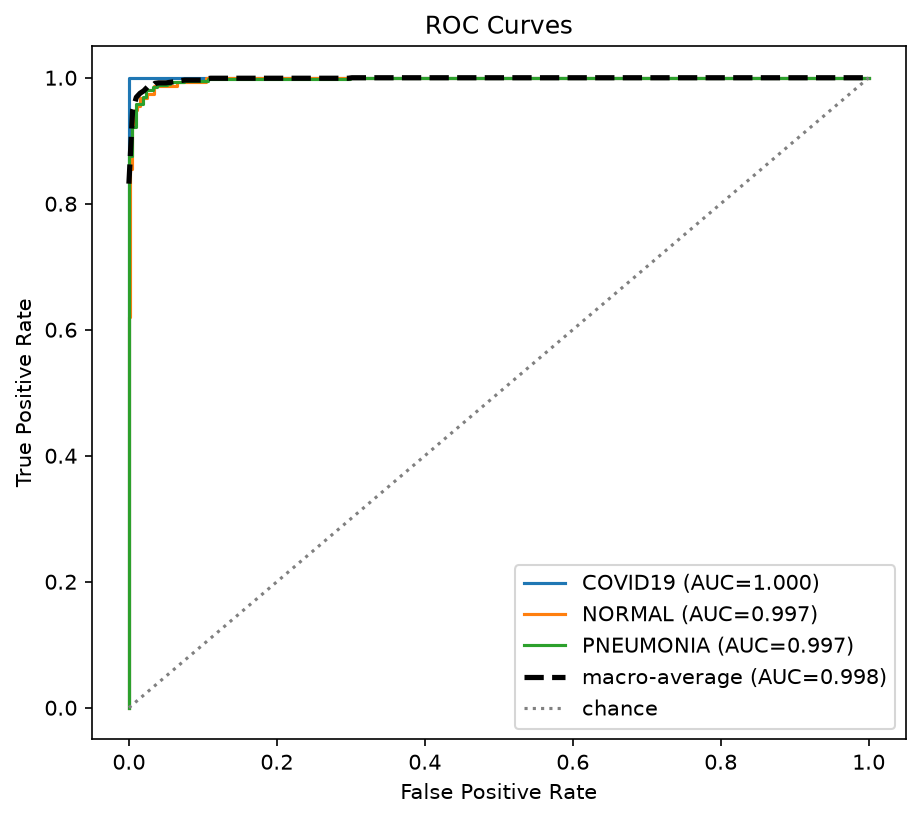
\includegraphics[width=\linewidth]{../results/figs/q1_roc.png}
\caption{One-vs-rest ROC}
\end{subfigure}
\caption{PneumoNet test-set performance.}
\label{fig:q1results}
\end{figure}

\begin{figure}[t]
\centering
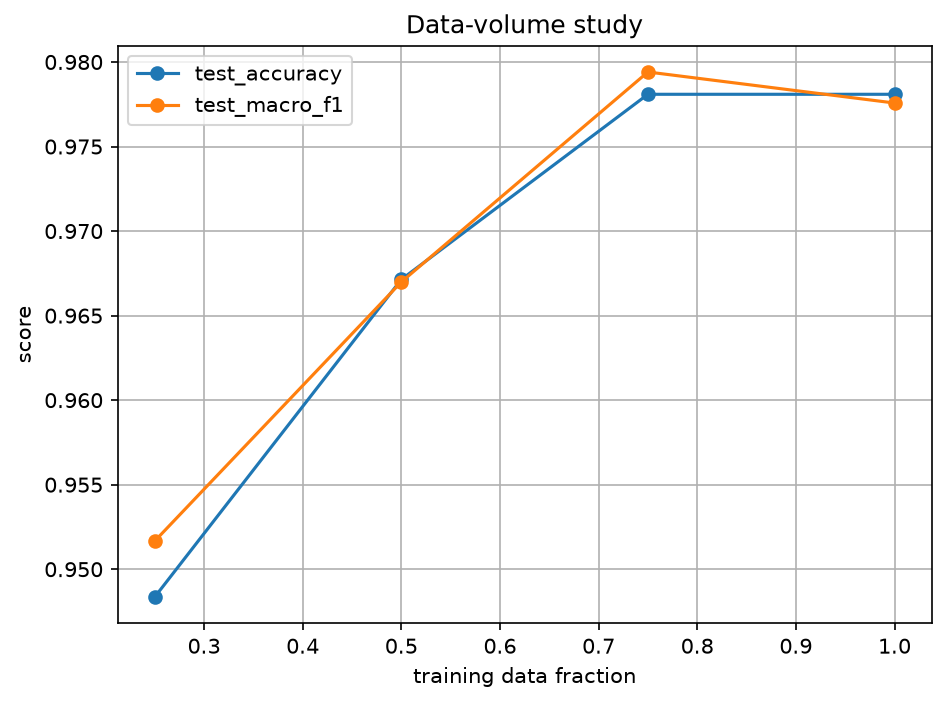
\includegraphics[width=0.85\linewidth]{../results/figs/q1_datavolume.png}
\caption{Test accuracy / macro-F1 vs. training-set fraction. Saturates at 75\%.}
\label{fig:datavol}
\end{figure}

\subsection{Q2}
The final configuration (teacher forcing 1.0, reversed source) reaches
best validation loss 3.9772 (perplexity 53.37) and test BLEU
\cite{papineni2002bleu} 4.64 over 844 held-out pairs --- an A/B/C
tuning result rather than a single run (Table~\ref{tab:q2tuning},
Section IV). Fig.~\ref{fig:q2curves} shows training/validation loss for
the final configuration, across its 18 epochs, falling well below the
untrained baseline $\ln(3{,}961)\approx8.28$.

\begin{figure}[t]
\centering
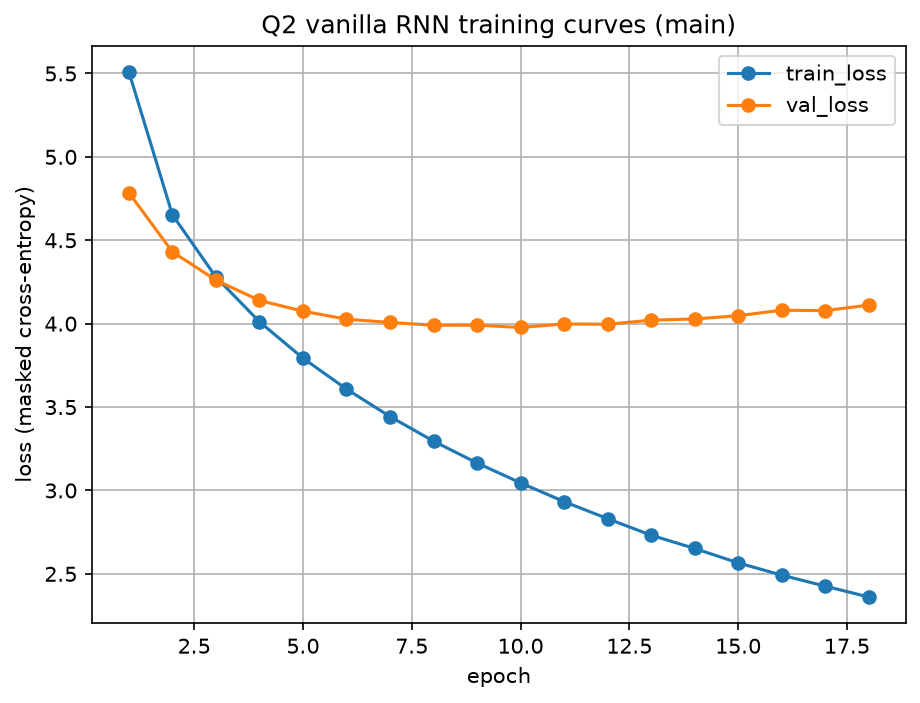
\includegraphics[width=0.85\linewidth]{../results/figs/q2_curves.png}
\caption{Q2 training/validation loss, final configuration, 18 epochs.}
\label{fig:q2curves}
\end{figure}

Length-bucketed test BLEU (Table~\ref{tab:q2lengthbucket}, fresh
samples in \texttt{results/q2\_samples.csv}) is close to flat across
source lengths, unlike the earlier configurations. Qualitatively, the
model produces fluent, register-appropriate Urdu at both short and long
source lengths, but that fluency does not imply faithfulness.
Table~\ref{tab:q2examples} shows the pattern: the model reproduces
Biblical register and anchors on individual content words, yet does not
compose a faithful translation. In the first example the opening clause
is reproduced exactly before the predicate diverges; in the second a
single content word survives while the rest of the proposition is lost.
Both patterns recur throughout \texttt{results/q2\_samples.csv}.

\begin{table*}[t]
\centering
\caption{Two test-set translations from the final configuration (teacher
forcing 1.0, reversed source). Glosses are literal back-translations of
the hypothesis.}
\label{tab:q2examples}
\footnotesize
\begin{tabular}{@{}p{0.26\textwidth}p{0.30\textwidth}p{0.38\textwidth}@{}}
\toprule
\textbf{Source} & \textbf{Reference} & \textbf{Hypothesis (gloss below)} \\
\midrule
blessed are the meek for they shall inherit the earth &
{\urdufont مبارک ہیں وہ جو حلیم ہیں کیونکہ وہ زمین کے وارث ہونگے} &
{\urdufont مبارک ہیں وہ جو خدا کے نزدیک ہے} \newline
``blessed are those who are near to God'' --- opening clause exact,
predicate wrong \\
\addlinespace
and he touched her hand and the fever left her &
{\urdufont اس نے اس کا ہاتھ چھوا اور تپ اس پر سے اتر گئی} &
{\urdufont اور وہ اس کے پاس آکر کہا کہ اس کو کس نے چھئوا دیا ہے} \newline
``and he came to him and said, who touched him?'' --- retains
\emph{touched}, loses the fever and the healing \\
\bottomrule
\end{tabular}
\end{table*}

\begin{table}[htbp]
\centering
\scriptsize
\caption{Q2 final-configuration test BLEU by source-length bucket.}
\label{tab:q2lengthbucket}
\begin{tabular}{lr}
\hline
Source length (tokens) & BLEU \\
\hline
1--5 & 4.343 \\
6--10 & 3.721 \\
11--15 & 3.315 \\
16+ & 4.125 \\
\hline
\end{tabular}
\end{table}


\section{Error Analysis and Discussion}

\subsection{Q1}
Only 13 of 639 test images are misclassified. By true class: COVID19
\textbf{0}, Normal 5, Pneumonia 8 --- zero errors on the rarest class
(56 test images), evidence the inverse-frequency-weighted loss is doing
its job rather than being swamped by the majority Pneumonia class.
Confusion is concentrated in the Normal/Pneumonia boundary
(Pneumonia$\to$Normal 7, Normal$\to$Pneumonia 5, Pneumonia$\to$COVID19
1). The model is also appropriately uncertain when wrong: mean
confidence is 0.853 on errors versus 0.989 on correct predictions, not
confidently wrong. Fig.~\ref{fig:errors} shows the 12
highest-confidence errors (of 13 total). These results are only honest
because of the BatchNorm fix in Section III: pre-fix, the frozen
baselines would have partly adapted to the domain via drifting running
statistics, inflating their scores and narrowing the frozen-vs-fine-tuned
gap this section reports as real. On regularization, dropout (0.3) did
the substantive work of controlling overfitting in the winning
configuration, while L2 was numerically inert over its searched range
(Section IV) and L1 measurably \emph{hurt} validation macro-F1
(0.9757 at $\lambda=0$ vs. 0.9665 at $\lambda=10^{-5}$) --- for this
model and this amount of data, explicit weight penalties added little
beyond what dropout and early stopping already provided.

\begin{figure}[t]
\centering
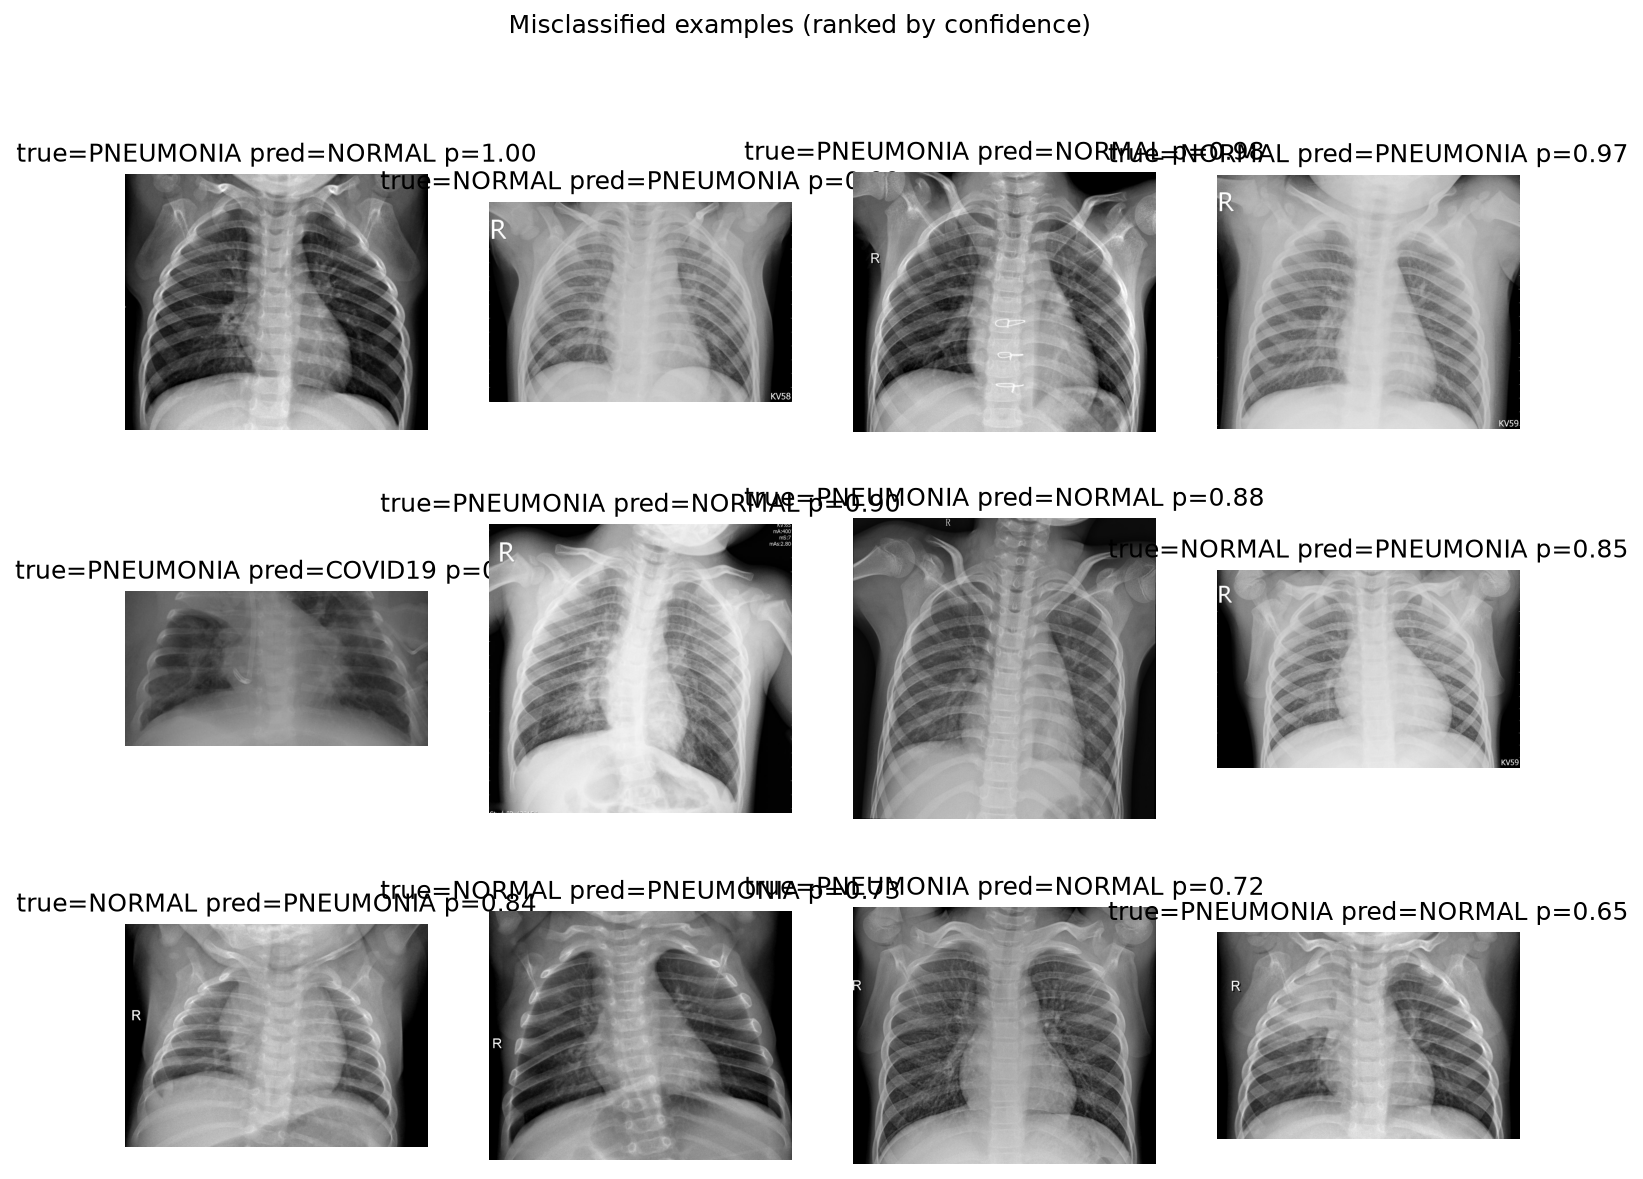
\includegraphics[width=\linewidth]{../results/figs/q1_errors.png}
\caption{Twelve highest-confidence Q1 misclassifications.}
\label{fig:errors}
\end{figure}

\subsection{Q2}
The error taxonomy (\texttt{results/q2\_error\_taxonomy.json}) over 844
test pairs, final configuration, shows UNK rate 12.88\%, repetition
rate 3.79\%, empty-output rate 0\%, and mean length ratio
(hypothesis/reference) 1.0544 --- the model now over-produces slightly
relative to the reference and still rarely degenerates into empty
output. Both the UNK rate and the repetition rate rose sharply from the
original, under-trained run (2.46\%$\to$12.88\% and
0.36\%$\to$3.79\% respectively) even as test BLEU nearly doubled
(Section IV): correcting under-training was not a uniform improvement
across metrics, and a configuration that wins on corpus-level n-gram
overlap can measurably lose on token-level degeneracy.

Length-bucketed BLEU is close to flat: 1--5 tokens 4.343, 6--10 tokens
3.721, 11--15 tokens 3.315, 16+ tokens 4.125
(Table~\ref{tab:q2lengthbucket}). This flattening is not a surprise but
a confirmation: source reversal shortens the dependency between early
source tokens and early target tokens (Section IV), so it should help
most exactly where the fixed-size hidden vector previously had the
furthest information to carry, i.e. the longer buckets --- which is
what the earlier length-degradation pattern reflected and reversal has
now removed.

A flat length curve does not mean the fixed-size-hidden-vector
limitation is gone; the evidence for it is now different, and stronger.
First, faithfulness: even the best configuration produces fluent,
domain-appropriate Urdu that is frequently unfaithful to the specific
source content rather than merely awkward (Section V examples) ---
consistent register, but wrong or absent propositional content.
Second, memorization: the model still cannot reliably reproduce
training pairs it has already seen repeatedly during training (32
times in the original diagnostic run, 18 times in the final
configuration), which is not a length or vocabulary-coverage problem
since these exact pairs have already been encountered many times over;
it is a sign that a single fixed-size hidden vector is not conditioning
generation strongly enough on the specific input, which is exactly the
bottleneck attention was introduced to remove
\cite{bahdanau2015attention}. The Q2 corpus's narrow, repetitive
Biblical domain (Section II) is precisely why this is visible: it lets
the model fall back on register-specific n-gram regularities that
sound right and score reasonably even when the content is wrong, so
fluency and raw BLEU understate the faithfulness gap, and neither BLEU
4.64 nor the flat length curve should be read as evidence the
bottleneck has been resolved.

\section{Conclusion and Future Work}

\subsection{Q1}
A 1.24M-parameter CNN trained from scratch, under a measured
preprocessing and augmentation policy and a corrected BatchNorm-freezing
implementation, outperforms fine-tuned VGG16 (108$\times$ the
parameters) and fine-tuned ResNet50 (19$\times$ the parameters) on
every held-out metric, with only 13 total misclassifications on the
test set. Limitations: the dataset is single-source and only 6,383
images after deduplication, chest radiographs across classes are
intrinsically visually correlated (Section II), and no external or
multi-institution validation was performed, so generalization beyond
this dataset's imaging protocol is unverified. Future work: multi-site
external validation, class-activation visualization (e.g. Grad-CAM) to
check the model attends to lung fields rather than markers or
positioning artifacts, and re-running the augmentation study with
anatomically valid transforms (small rotations, intensity jitter)
rather than horizontal flips.

\subsection{Q2}
Once an under-trained teacher-forcing schedule and a forward-only
source order were diagnosed and corrected (test BLEU 2.45$\to$4.64;
Section IV), the vanilla RNN encoder--decoder still shows the
limitation this study set out to measure, just via different evidence
than originally reported: even its best configuration produces fluent,
domain-appropriate Urdu that is frequently unfaithful to the source and
still cannot reliably reproduce training pairs it has seen repeatedly,
indicating the single fixed-size hidden vector it must pass from
encoder to decoder under-conditions generation on the specific input
(Section VI) rather than merely truncating long sentences. Limitations:
the corpus is 9,103 pairs, not the assignment's stated $\sim$24,000,
and is domain-narrow and repetitive (Section II), so these results
should not be read as general-purpose English--Urdu translation
quality; the corrected configuration also raised the UNK and repetition
rates even as BLEU improved, so the fix is a net gain, not a uniform
one. The named remedy, evidenced rather than assumed, is architectural:
adding an attention mechanism \cite{bahdanau2015attention} so the
decoder can access all encoder states instead of one bottleneck vector,
or replacing \texttt{nn.RNN} with a gated unit (LSTM/GRU) to improve
long-range gradient flow, would directly target the faithfulness gap
this study measured. Future work also includes sourcing a larger,
general-domain parallel corpus so results are comparable to the
published NMT literature.

\begin{thebibliography}{9}
\bibitem{simonyan2015vgg} K. Simonyan and A. Zisserman, ``Very Deep Convolutional Networks for Large-Scale Image Recognition,'' \emph{ICLR}, 2015.
\bibitem{he2016resnet} K. He, X. Zhang, S. Ren, and J. Sun, ``Deep Residual Learning for Image Recognition,'' \emph{CVPR}, 2016.
\bibitem{ioffe2015batchnorm} S. Ioffe and C. Szegedy, ``Batch Normalization: Accelerating Deep Network Training by Reducing Internal Covariate Shift,'' \emph{ICML}, 2015.
\bibitem{sutskever2014seq2seq} I. Sutskever, O. Vinyals, and Q. V. Le, ``Sequence to Sequence Learning with Neural Networks,'' \emph{NeurIPS}, 2014.
\bibitem{bahdanau2015attention} D. Bahdanau, K. Cho, and Y. Bengio, ``Neural Machine Translation by Jointly Learning to Align and Translate,'' \emph{ICLR}, 2015.
\bibitem{papineni2002bleu} K. Papineni, S. Roukos, T. Ward, and W.-J. Zhu, ``BLEU: a Method for Automatic Evaluation of Machine Translation,'' \emph{ACL}, 2002.
\bibitem{loshchilov2019adamw} I. Loshchilov and F. Hutter, ``Decoupled Weight Decay Regularization,'' \emph{ICLR}, 2019.
\end{thebibliography}

\end{document}
